\documentclass[11pt,a4paper]{article}  % Déclare la classe du document.

\newcommand{\chaptermark}[2]{\og #2 \fg{} (#1)} % ligne uniquement pour éviter une erreur en cas d'article
\include{../1ere-preambule}

\usepackage{epic}   % extension et simplification de  l'environnement picture
\usepackage{graphicx}    % permet d'inclure des graphique externe dans un document
\usepackage{arydshln}   %permet d'avoir des lignes en pointillés

\newcommand{\lignes}[1]{
	\setlength{\unitlength}{1mm}
	\vskip 0,4cm\noindent
	\multido{\i=0+1}{#1}{%
		\noindent
		\begin{picture}(150,5)
			\linethickness{0,005mm}
			\put(-5,0){\dashline{1}(175,5)(5,5)}
		\end{picture}\vskip 0,001cm
	}
	\vskip 0cm
}

\rhead{\textcolor{red}{Correction $-$ Préparation Bac Blanc $-$ 20/01/2026}}

\newcommand{\va}[1]{\lvert \ #1 \ \rvert}
\newcommand{\vaf}[1]{\left\lvert \ #1\  \right\rvert}

\begin{document}
	\graphicspath{{images/}}
	
	\begin{center}
		
		
		\fbox{
			\begin{minipage}[]{15cm}
				\begin{center}
					\LARGE{\rule{0.5cm}{0pt}\rule[-0.25cm]{0pt}{0.9cm}
						\textcolor{red}{Correction $-$ Préparation au bac blanc}
					}
				\end{center}
			\end{minipage}
		}
	\end{center}

%\begin{center}\textbf{Durée 2h $-$ Barême indicatif}\end{center}
%\begin{center}\textbf{Les élèves avec un tier-temps ne traitent pas les questions avec  le symbole \ding{46}}\end{center}
%\begin{center}\textbf{Calculatrice non autorisée.\\Les résultats devront être justifiés (à l'aide de calcul ou de propriétés).}\end{center}


\exerciceDS{ $-$ QCM sur les automatismes.}

Pour chacune des six questions suivantes, une seule réponse est exacte. Laquelle ? L'entourer directement sur cette feuille.

\begin{enumMet}
	\item Augmenter une valeur de $20 \%$ revient à multiplier cette valeur par :
	\begin{multicols}{4}
	\begin{enumMet}
		\item 	0,2
		\item 0,8
		\item \fbox{1,2}
		\item 1,02
	\end{enumMet}
	\end{multicols}
	\begin{corrBox}
		$c=1+t=1+\dfrac{20}{100}=1+0,2=1,2$		
	\end{corrBox}
	\item Le prix d'un pantalon a augmenté de $25 \%$ en 2025 . Pour retrouver sa valeur initiale, le nouveau prix doit être baissé de :
	\begin{multicols}{4}
		\begin{enumMet}
		\item \fbox{20 \%}
		\item 25 \%
		\item 30 \%
		\item 75 \%
	\end{enumMet}
	\end{multicols}
	\begin{corrBox}
		$c=1+t=1+\dfrac{25}{100}=1+0,25=1,25\longrightarrow\dfrac{1}{1,25}=\dfrac{100}{125}=\dfrac{100\div25}{125\div25}=\dfrac{4}{5}=0,8=1-\dfrac{20}{100}$		
	\end{corrBox}
	\item L'équation $5 x-6=9$ a pour ensemble solution dans $\mathbb{R}$ :
	\begin{multicols}{4}
		\begin{enumMet}
			\item $S=\{5\}$
			\item \fbox{$S=\{3\}$}
			\item $S=\left\{\frac{3}{5}\right\}$
			\item $S=\{-3\}$
		\end{enumMet}
	\end{multicols}
	\begin{corrBox}
		$5 x-6=9\iff 5x=9+6\iff 5x=15\iff x=\dfrac{15}{5}\iff x=3$		
	\end{corrBox}
	\item L'expression affine $\mathrm{A}(x)=-2 x+8$ a pour tableau de signes :
	\begin{multicols}{2}
		\begin{enumMet}
		\item \begin{tikzpicture}
			\tkzTabInit[lgt = 1.5, espcl = 1.7]{$x$ / 1 , $A(x)$ / 1}{$-\infty$, $4$, $+\infty$}
			\tkzTabLine{, +, z, -, }
		\end{tikzpicture}	
		\item \begin{tikzpicture}
			\tkzTabInit[lgt = 1.5, espcl = 1.7]{$x$ / 1 , $A(x)$ / 1}{$-\infty$, $4$, $+\infty$}
			\tkzTabLine{, -, z, +, }
		\end{tikzpicture}	
		\item \begin{tikzpicture}
			\tkzTabInit[lgt = 1.5, espcl = 1.7]{$x$ / 1 , $A(x)$ / 1}{$-\infty$, $-4$, $+\infty$}
			\tkzTabLine{, +, z, -, }
		\end{tikzpicture}	
		\item \begin{tikzpicture}
			\tkzTabInit[lgt = 1.5, espcl = 1.7]{$x$ / 1 , $A(x)$ / 1}{$-\infty$, $-4$, $+\infty$}
			\tkzTabLine{, -, z, +, }
		\end{tikzpicture}	
	\end{enumMet}
	\end{multicols}
	\begin{corrBox}
		On résoud $A(x)=0\iff -2x+8=0\iff -2x=-8\iff x=\dfrac{-8}{-2}=4$. De plus la fonction $A(x)$ est une fonction affine avec m<0 (coefficient directeur). Elle est donc strictement décroissante et d'abord positive et ensuite négative. Elle change de signe pour x=4. Solution a
		
		\begin{tikzpicture}
			\tkzTabInit[lgt = 1.5, espcl = 1.7]{$x$ / 1 , $A(x)$ / 1}{$-\infty$, $4$, $+\infty$}
			\tkzTabLine{, +, z, -, }
		\end{tikzpicture}	
	\end{corrBox}
	 \item La forme factorisée de l'expression algébrique $f(x)=x-4 x^{2}$ est :
	\begin{multicols}{4}
		\begin{enumMet}
			\item a) $f(x)=x(-4 x)$
			\item $f(x)=-4 x^{2}$
			\item $f(x)=-4 x$
			\item \fbox{$f(x)=x(1-4 x)$}
		\end{enumMet}
	\end{multicols}
	\begin{corrBox}
			$f(x)=x-4 x^{2}=\underline{x}\times 1-4x\times \underline{x}=x(1-4x)$		
	\end{corrBox}
	\item L'ensemble des solution de l'équation $(x-7)(5 x+4)=0$ est :
	\begin{multicols}{4}
		\begin{enumMet}
			\item\fbox{$\left\{7\ ;\ -\dfrac{4}{5}\right\}$}
			\item $\{7\ ;\ 0,8\}$
			\item $\left\{-7\ ;\ -\dfrac{4}{5}\right\}$
			\item $\{-7\ ;\ 0,8\}$
		\end{enumMet}
	\end{multicols}
	\begin{corrBox}
		Equation Produit nul.
		
		$x-7=0$ ou $5x+4=0$
		
		$x=7$ ou $5x=-4$
		
		$x=7$ ou $x=-\dfrac{4}{5}$
				
	\end{corrBox}
\end{enumMet}

%\newpage
\exerciceDS{}

En 2024, un club de boxe compte 94 adhérents. On considère que chaque année l'effectif du club augmente de 4 adhérents. Pour tout entier naturel $n$, on note $a(n)$ le nombre d'adhérents au club de boxe pour l'année $2024+n$.
\begin{enumMet}
	\item Compléter directement sur cette feuille : $a(0)=$\quad\corr{$94$}
	\item Calculer $a(1)$ et écrire une phrase qui explique ce que représente $a(1)$
	\begin{corrBox}
		$a(1)=a(0)+4=94+4=98$. En $2025$, le club comptera 98 adhérents.		
	\end{corrBox}
	\item \begin{enumMet}
		\item Donner la relation de récurrence de la suite $a$ qui exprime, pour tout entier naturel $a, a(n+1)$ en fonction de $a(n)$
		\begin{corrBox}
			$a(n+1)=a(n)+4$		
		\end{corrBox}
		\item En déduire la nature de cette suite.
		\begin{corrBox}
			Pour passer d'un terme de la suite à l'autre, on ajoute toujours la même chose (4). Il s'agit donc d'une suite arithmétique de raison $r=4$		
		\end{corrBox}
	\end{enumMet}
	\item En déduire l'expression, pour tout entier naturel $n$, de $a(n)$ en fonction de $n$
	\item En déduire le nombre d'adhérents du club en 2030 que l'on peut estimer avec ce modèle.
	\item Compléter l'algorithme ci-dessous (directement sur le sujet) afin qu'il affiche au bout de combien d'années la population de cette ville devient supérieure ou égal à 120 adhérents.\\
	(Toujours en utilisant le même modèle d'évolution de population)
	\begin{verbatim}
		N=0
		U=94
		while U ......
					U=........
					N=N+1
		print(N)
	\end{verbatim}
\end{enumMet}

\exerciceDS{}

Ewan a une collection de 150 mangas et bandes dessinées.

Dans sa collection， $20 \%$ abordent le thème de la comédie et $50 \%$ celui de la science-fiction．

De plus， $70 \%$ de sa collection est composée de mangas. $40 \%$ de ses mangas traitent de science-fiction. Les comédies sont réparties équitablement entre mangas et BD.

\begin{enumMet}
	\item Parmi les 150 mangas et bandes dessinées que possède Ewan, combien abordent le thème de la comédie?
	\item De combien de mangas est composée la collection d'Ewan?
	\item Recopier et compléter le tableau suivant:
	
	\begin{tabular}{|l|l|l|l|l|}
		\cline { 2 - 5 } \multicolumn{1}{c|}{} & Aventure & Comédie & Sc. fiction & Total \\
		\hline Manga & & & & \\
		\hline BD & & & & \\
		\hline Total & & & & \\
		\hline
	\end{tabular}
	\item Quelle est la fréquence $f$ de BD ayant comme thème l'aventure?
	\item Parmi les Livres ayant comme thème l'aventure, quel est le pourcentage de BD?\\
\end{enumMet}


\newpage
\exerciceDS{}

Le responsable d'une plateforme de vente en ligne de vêtements d'occasion a réalisé une étude concernant l'évolution du nombre de vendeurs (offre) et du nombre d'acheteurs (demande) en fonction du prix de vente d'un T-shirt à édition limitée puis il a réalisé le graphique ci-dessous.
\ \\

\begin{center}
\begin{tikzpicture}%
	[x=0.16cm,y=0.16cm, %unités
	xmin=0,xmax=100,xgrille=10,xgrilles=5, %axe Ox
	ymin=0,ymax=50,ygrille=10,ygrilles=5] %axe Oy
	\GrilleTikz
	\AxesTikz%
	[AffLabel=xy,Labelx={Nombre de T-shirts},Labely={Prix (en \EUR{})},%
	PosLabelx={below left},PosLabely={above right},%
	Police=\small\sffamily,ElargirOx=0,ElargirOy=0]
	\AxexTikz[Police=\small]{0,10,...,80}
	\AxeyTikz[Police=\small]{0,10,...,40}
	\CourbeTikz[line width=1.4pt,ForestGreen,samples=250]%
	{-0.5*\x+50}{0:100} %courbe
	\draw (90,10) node[color=ForestGreen] {Demande};
\end{tikzpicture}
\end{center} 

\begin{enumMet}
	\item On rappelle que la fonction \guillemets{offre} est définie sur [10; 70] par $g(x)=0,5x+15$
	\begin{enumMet}
		\item Pour un prix de vente de $40$ \EUR{} à combien d'article correspond l'offre ?
		\item Calculer $g(40)$. Que représente ce résultat ?
		\item Sur le graphique ci-dessus et à l'aide des calculs précédents, tracer la représentation graphique de la fonction « demande » $g$.
	\end{enumMet}
	\item On rappelle que la fonction affine \guillemets{demande} $f$ définie sur $[10 ; 100]$ est représentée en verte sur le graphique ci-dessus.
	\begin{enumMet}
		\item Lire graphiquement et compléter la réponse directement sur cette feuille $f(20)=\ldots$
		\item Pour cette question seulement on considère que le prix de vente est fixé à $30$ \EUR{}.
		
		Graphiquement déterminer la demande des consommateurs correspondante.
		\item Déterminer le coefficient directeur de la droite représentant la fonction \guillemets{demande}.
		
		On justifiera à l'aide d'une formule.
		\item Déterminer l'expression de la fonction $f$.
	\end{enumMet}
	\item \begin{enumMet}
		\item Résoudre $0,5x+15=-0,5 x+50$
		\item On dit que le marché est à l'équilibre lorsque, pour un même prix, la quantité offerte est égale à la quantité demandée.
		
		En déduire le prix d'équilibre et la quantité associée.
	\end{enumMet}
	
\end{enumMet}





\end{document}
